\chapter{Einleitung}
\label{chap:einleitung}

\begin{figure}[h]
	\centering
	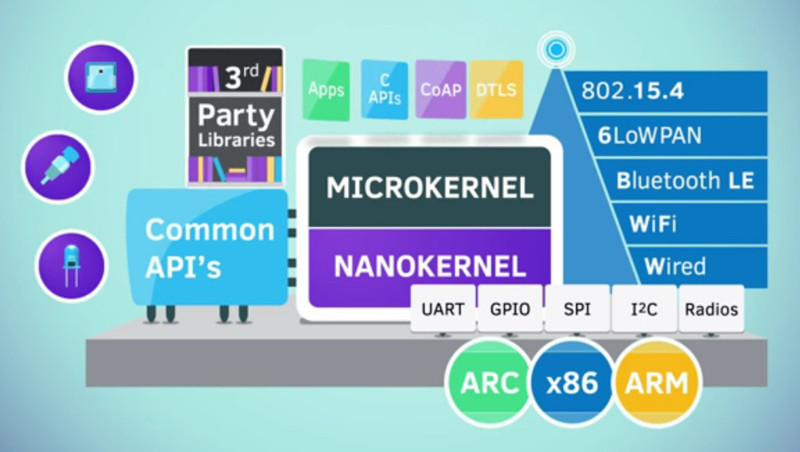
\includegraphics[width=0.7\linewidth]{bilder/zephyr_components.jpg}
	\caption{Komponenten und Übersicht über das Zephyr RTOS}
	\label{fig:components}
\end{figure}

In dieser Projektarbeit soll zuerst ein Vergleich der Eigenschaften ähnlicher
Betriebssysteme wie FreeRTOS, RIOT, Kontiki, usw. vor allem bezüglich der Unterstützung der
verschiedenen Netzwerkprotokolle gemacht werden. Im Fokus steht dabei das n
Zu Demonstrationszwecken soll am Schluss mit dem ausgewählten Board eine Demo-App entwickelt werden.

Die Ziele sind:

\begin{itemize}
	\item Einarbeitung in das Betriebssystem Zephyr.
	\item Erstellen einer Vergleichstabelle mit den wichtigsten Eigenschaften der verschiedenen
	RTOS.
	\item Evaluation geeigneter Boards für das Zephyr Betriebssystem für eine IoT
	\item Entwicklung einer Demonstrationsapplikation, basierend auf dem ausgewählten Board
\end{itemize}